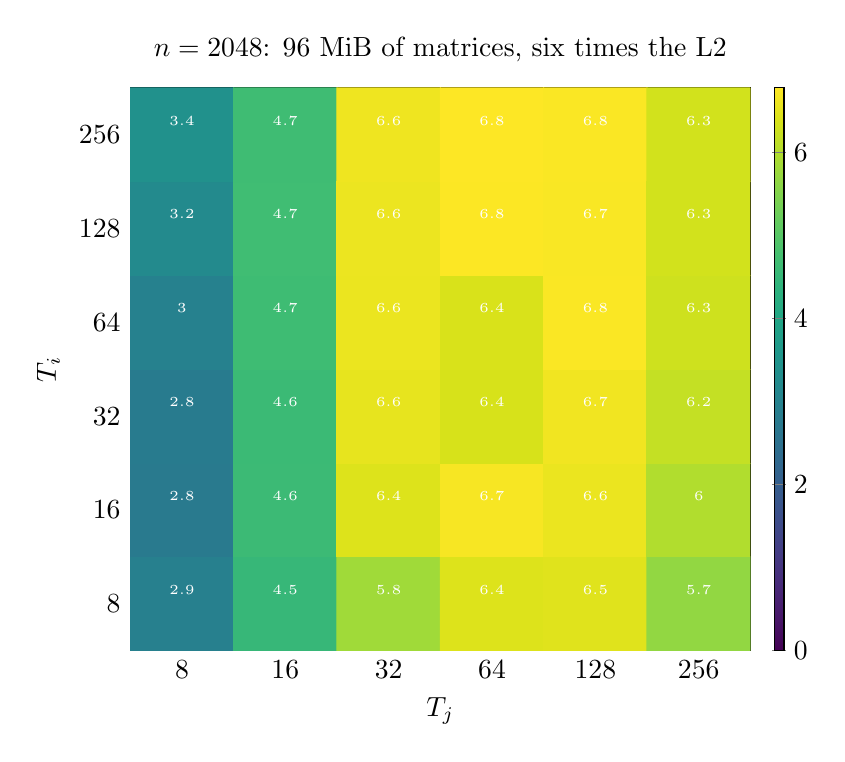
\begin{tikzpicture}
\begin{axis}[width=0.78\linewidth, height=0.72\linewidth, view={0}{90}, colorbar, colorbar style={width=0.12cm, ytick={0,2,4,6,8}, ylabel={}}, colormap/viridis, xlabel={$T_j$}, ylabel={$T_i$}, title={$n=2048$: 96 MiB of matrices, six times the L2},
  xtick={0,...,5}, xticklabels={8,16,32,64,128,256}, ytick={0,...,5}, yticklabels={8,16,32,64,128,256},
  enlargelimits=false, point meta min=0, nodes near coords={\pgfmathprintnumber[precision=1]{\pgfplotspointmeta}}, nodes near coords style={font=\tiny, white}]
\addplot[matrix plot*, point meta=explicit, mesh/cols=6] coordinates {
(0,0) [2.93]
(1,0) [4.53]
(2,0) [5.82]
(3,0) [6.44]
(4,0) [6.47]
(5,0) [5.68]
(0,1) [2.76]
(1,1) [4.62]
(2,1) [6.44]
(3,1) [6.71]
(4,1) [6.59]
(5,1) [6.00]
(0,2) [2.80]
(1,2) [4.61]
(2,2) [6.55]
(3,2) [6.38]
(4,2) [6.65]
(5,2) [6.19]
(0,3) [2.96]
(1,3) [4.66]
(2,3) [6.59]
(3,3) [6.40]
(4,3) [6.75]
(5,3) [6.29]
(0,4) [3.21]
(1,4) [4.69]
(2,4) [6.60]
(3,4) [6.77]
(4,4) [6.74]
(5,4) [6.33]
(0,5) [3.42]
(1,5) [4.67]
(2,5) [6.63]
(3,5) [6.78]
(4,5) [6.75]
(5,5) [6.33]
};
\end{axis}
\end{tikzpicture}